%% LyX 2.2.3 created this file.  For more info, see http://www.lyx.org/.
%% Do not edit unless you really know what you are doing.
\documentclass[10pt,a4paper]{article}
\usepackage[utf8]{inputenc}
\setcounter{secnumdepth}{3}
\setcounter{tocdepth}{3}
\usepackage{amsmath}
\usepackage{amssymb}
\usepackage{algorithm2e}
\usepackage{mathtools}
\usepackage{enumitem}
\usepackage{float}
\usepackage{graphicx}
\usepackage{caption}

\makeatletter

%%%%%%%%%%%%%%%%%%%%%%%%%%%%%% LyX specific LaTeX commands.
\special{papersize=\the\paperwidth,\the\paperheight}
\addtolength{\oddsidemargin}{-70pt}
\addtolength{\textwidth}{150pt}

%%%%%%%%%%%%%%%%%%%%%%%%%%%%%% User specified LaTeX commands.
\usepackage{amsfonts}
\usepackage{amsthm}
\usepackage{relsize}
\DeclareMathOperator*{\argmax}{argmax}
\DeclareMathOperator*{\argmin}{argmin}
\newcommand{\defeq}{\mathrel{\overset{\makebox[0pt]{\mbox{\normalfont\tiny\sffamily def}}}{=}}}
\renewcommand{\thesubsection}{\alph{subsection}.}


\makeatother

\begin{document}

\title{NLP - 097215 - Computer Exercise No. 2}
\maketitle
\subsection{Submitted by:}
Avrech Ben-David - 200452282\\
Ilan Frank - 043493386

\subsection{Training}
We implemented a dependency parser based on McDonald 2005.
Besides the unigram and bigram features required in the exercise (for model 1), we added additional
features to the complex model (model 2). These features include:

\begin{itemize}[leftmargin=*]
\item 14: $dist(h,m)$: The distance in words between parent and child nodes.
\item 15: (p-pos, p-next-pos): where p-next-pos is the part of speech following the p node.
\item 16: (p-pos, c-pos, $dist(h,m)$): combined feature for parent and child nodes with the distance between them.
\item 17: $len(sentence)$: where we took the actual length of the sentence for sentences under 30 words, the floor length to the nearest tens digits for sentences between 30 and 100 (i.e., 48 goes to 40) and the hundreds digit for sentences above 100 (217 goes to 200).
\item 18: (c-pos, c-next-pos, p-pos) if the distance between the parent and child is greater than 1.
\end{itemize}

The basic feature set for model 1 achieved poor performance. The test accuracy upper bound was around 0.3. We analyzed the confusion matrix of model 1, and noticed that there are common mistakes which the parent POS was predicted correctly, but the distance between the child and parent was wrong. This was the motivation to introduce distance based features 14-17. 

We generated the features for all positive occurrences in our train set, and in addition, to give the model more degrees of freedom, we generated the features (p-pos, c-pos) (feature 13), and features 15, 16 for unobserved combinations - for all POS combinations and for distances in range [-20:20]. The unobserved features, are subtracted from the weight vector when an error occours, so in the next time such a false candidate will get a lower score.

The addition of features 14-17 achieved test accuracy of 0.78. We further analyzed the confusion matrix, and revealed that a considerable mass of the errors occur when the model predict a parent which is far from the child, while the true parent actually follows the child. We added additional "punishment" feature (18), that punishes false predictions such that. This last feature improved the test accuracy to stand on 0.8 after a small number of epochs.

We also examined thresholding the sparsed features (4,8,10) in order to accelerate training. In fact, thresholding did not shorten the training time significantly, but the performance seemed to be slightly worse, so we discarded this option. 

Table \ref{tab:feature-set-summary} lists the number of features for each model.
\begin{table}[htb]
\centering
\begin{tabular}{|c|c|c|}

\hline Feature ID & Model 1 &  Model 2 \\ 
\hline 1          & 9993    &  9993    \\       
\hline 2          & 8876    &  8876    \\       
\hline 3          & 37      &  37      \\       
\hline 4          & 15908   &  15908   \\       
\hline 5          & 14162   &  14162   \\       
\hline 6          & 45      &  45      \\       
\hline 7          & 0       &  0       \\       
\hline 8          & 31314   &  31314   \\       
\hline 9          & 0       &  0       \\       
\hline 10         & 33936   &  33936   \\       
\hline 11         & 0       &  0       \\       
\hline 12         & 0       &  0       \\       
\hline 13         & 1441    &  1441    \\       
\hline 14         & 0       &  126     \\       
\hline 15         & 0       &  1433    \\       
\hline 16         & 0       &  58469   \\       
\hline 17         & 0       &  38      \\       
\hline 18 		  & 0       &  1639    \\       
\hline Total      & 115712  &  177417  \\
\hline
\end{tabular}
\caption{Feature-Set Summary}
\label{tab:feature-set-summary}
\end{table}

\subsection{Inference}
Inference was made using the supplied Chu-Liu-Edmonds algorithm, with a score function based on the local and global features of the sentence.

\subsection{Test}
We trained each model for 20, 50, 80 and 100 epochs as required. The train and test accuracy are reported in table \ref{tab:100epochs-acc} as well as the training time. These training sessions ran on Asus UX305L with intel i5, and 8GB RAM. The training time is not consistent with the model size for unknown reason.

\begin{table}[htb]
\centering
\begin{tabular}{|c|c|c|}
\hline Epoch      			& Model 1 	& Model 2    \\ 
\hline 20          			& 0.31    	& 0.77       \\       
\hline 50          			& 0.3      	& 0.78       \\       
\hline 80          			& 0.3     	& 0.77       \\       
\hline 100                  & 0.31    	& 0.77       \\       
\hline Training Time       	& 233[min]  & 202[min]   \\
\hline Inference Time      	& 30.6[sec] & 31.2[sec]  \\
\hline
\end{tabular}
\caption{Test Accuracy for Both Models.}
\label{tab:100epochs-acc}
\end{table}

Actually, we achieved the best accuracy on the test set after 14 epochs. After this point the model accuracy reaches a plateau. The program output is presented in figure \ref{fig:m2-best-results}. We ran this session on Asus X510U with 8GB RAM and NVIDIA 930MX, but the GPU was idle most of the time. 

\begin{figure}
  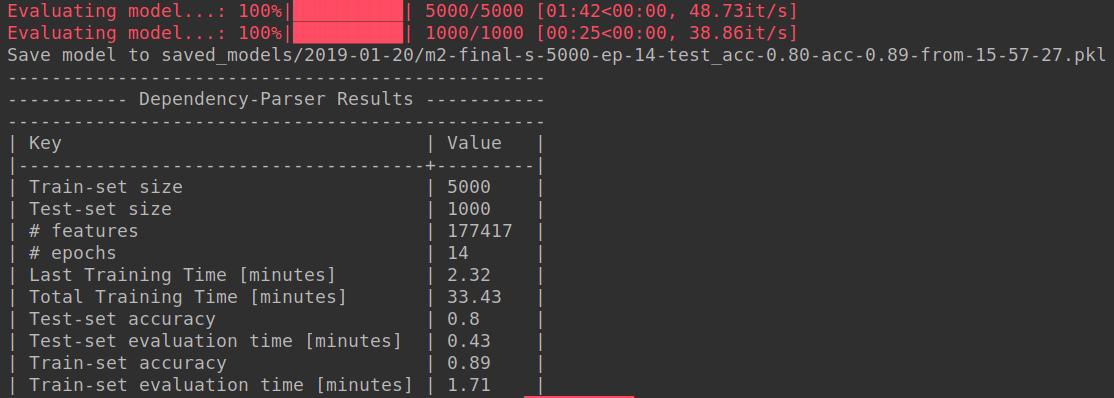
\includegraphics[width=\linewidth]{m2-final-ep-14-test-acc-08.jpg}
  \caption{Model 2 Test Results}
  \label{fig:m2-best-results}
\end{figure}


\subsection{Competition}
We used the complex model to annotate the competition file. Model 2 was freezed after epoch 14, the first epoch with the maximal test accuracy. We chose this snapshot in order to avoid the overfitting to the train set. We predict an accuracy of around 0.75. Actually we used the test set as a validation set. the extended features were selected in order to avoid the model mistakes as they were reflected in the test confusion matrix. If the competition set distribution is significantly different, it could results in inferior performance. Anyway, we saw that the sentences length is mainly shorter in the competition file, so we are still optimistic.
 
\subsection{Work Partition}
One team member was responsible for the training and inference skeleton. The other was responsible for  managing model versions and results analysis. Both members contributed to the feature generation. 

\subsection{Results Reproduction}
To reproduce our results, follow the instructions in the supplied README file. The README file contains commands for installation of compatible python3 virtualenv, and instructions for running our code.

\end{document}
